\section{Introduction}

%\subsection{Problem Statement \redtext{(what is the problem to be solved?)}}
%We develop a centralized method for estimating missing data in sensor network datasets, a procedure which is crucial for subsequent analysis.
%Missing data imputation (a term from Statistics) has a long history, and while there are many existing algorithms which estimate missing sensor data (as documented in Section \ref{sec:rw}), few of these take advantage of the time and inter-sensor correlations inherent in the WSN datasets.
%Furthermore, distributed approaches~\cite{xiao2006space,nowak2003distributed} are often limited to providing estimations or decisions based on sensors in the immediate neighborhood and rely on the deployed sensors having adequate computational power to perform such calculations.
%Not suffering from these issues, the centralized approach we have taken enables a global solution (utilizing all observations available from the sensor network) and provides a vital backdrop for our novel highly-accurate sensor network data imputation technique.

%\subsection{Relevance (why is WSN dataset analysis an important topic?)}
%The increasing pervasiveness of Wireless Sensor Network (WSN) deployments is reflected by the recent coinage of terms such as ``Internet of Things'' and ``Machine-to-Machine'' to describe this growing revolution~\cite{ashton2009internet,gershenfeld2004internet,nokia2004machine,lawton2004machine}.
%Facilitated by a sharp reduction in hardware costs~\cite{estrin2000special}, this growing trend (beyond providing for the admission of new phrases into the vernacular) has led to an explosion in the amount and variety of sensor network todata in need of study.
%For this reason, analysis of WSN data has garnered much attention in recent years~\cite{balazinska2007data}.

%\subsection{Motivation \redtext{(why is data imputation needed for WSN datasets?)}}

% Data sets gathered from sensor networks often suffer from a significant fraction of missing data, due to issues such as 
% communication interference, sensor interference, power depletion, and hardware failure. 
% Many standard data analysis tools such as classification engines, time-sequence pattern analysis modules, and even statistical tools are ill-equipped to deal will missing values---hence, there is a need to impute missing readings prior to analysis.

Wireless sensor networks (WSNs) are especially susceptible to interference,
battery depletion, hardware failures, and other environmental and communications ailments
that lead to data loss.  Datasets gathered from sensor networks are
often missing a significant fraction of the possible readings
(e.g., the Intel Berkeley Research lab dataset~\cite{berkeley2004lab}
is missing roughly 50\% of its readings).
These missing values are problematic for data analysis tools such as
classification engines, time-sequence pattern analysis modules, and
other machine learning tasks, which are often ill-equipped to deal
with missing values.  Support Vector Machine
(SVM)~\cite{vapnik2000nature} and Multiple Regression (MR) analysis,
to name but a few examples, require complete datasets with no missing
values.  Popular statistical packages such as SAS, Stata, and R
provide a few default options for handling missing data, as a
preprocessing step, because the core algorithms require that all data be filled
in.  Typical options are (i) remove the entire ``column'' if there is a
missing value or (ii) fill in the missing value (called {\em
imputation}) using either simple defaults like the average of
neighboring values or utilizing user-written code.  The first option discards
otherwise useful data, and in fact, may discard most of the columns in
datasets with high data loss.  Thus, imputation is a vital tool in the
preparation of sensor data for subsequent analysis. Because the
accuracy of the target data analysis depends on the accuracy of the
imputation, improvements in sensor data imputation can better serve
sensor network deployment objectives.

%We consider the common setting where the goal is to collect all the sensor readings
%in order to perform centralized analysis, while maximizing the lifetime of the WSN.
%Sensor nodes are battery powered and may be energy-harvesting, and will often make
%only a ``best effort'' attempt to transmit their readings back to the centralized 
%collection point.  This contributes to the prevalence of missing data, furthering
%the value of effective imputation techniques.

%\subsection{Background \redtext{(what solutions currently exist?)}}

\subsection{Existing Imputation Techniques} \label{sec:existing_work}

Imputation techniques applied to sensor data can be divided into three categories by the information utilized:
temporal methods (i.e., estimation using the observations from the target sensor at nearby time steps), 
spatial methods (i.e., estimation using neighboring sensor node observations), 
and spatio-temporal methods. They can be further categorized as hot-deck imputation and prediction models~\cite{Garcia:KNNreview},
as shown in Table~\ref{tbl:methods}.
%Hot-deck imputation methods directly fill in the missing values using either neighbor values or historical records from itself 
%such as the \textit{last-seen} method, while the prediction models exploit a function (involving metrics other than just sensor 
%values) to estimate the missing values. 

%The feasibility of estimating missing sensor observations based on historical data is grounded by the known temporal correlation in WSN data~\cite{akyildiz2004exploiting}.
%Moreover, where there is a potential for global communication issues to affect the availability for sensor node observations \emph{en masse} during a given duration of time, utilizing spatial correlations as a basis for estimation may be not be possible.

\paragraph{Temporal Methods}
{\em Temporal methods} leverage the temporal correlation among
readings by the same sensor node; salient methods include observed
data mean~\cite{madden2005tinydb}, last
seen~\cite{Granger:lastseen}, and linear interpolation. %:
%the estimated value $\hat{y_{it}}$ for sensor $i$ at time $t$ is
%$\hat{y_{it}} = y_{iu} + \frac{y_{iv}-y_{iu}}{T_v-T_u}(t-T_u)$,
%where $y_{iu}$ ($y_{iv}$) at time $T_u$ ($T_v$) is the first 
%observation for sensor $i$ prior to (after, respectively) time $t$.

These methods
suffer, however, when there are long temporal gaps in observations for a given
sensor; such gaps can be frequent in WSNs due to power depletion in
energy-harvesting sensors, long-lived communication ailments, etc.  
As a result, the usefulness of temporal imputation
methods drops rapidly as the number of consecutively missing readings
becomes large.

% (i.e., as can happen when intermittent communications starvation occurs in large WSNs).  

\begin{table}
\caption{Salient Methods for Sensor Data Imputation}
\label{tbl:methods}
\centering
{\small
\begin{tabular}{|l|l|l|} \hline
   &{\bf Hot-Deck Imputation}&{\bf Prediction Models}\\ \hline
{\bf Temporal} & Last-seen~\cite{Granger:lastseen}, Mean& Linear Interpolation\\ \hline
\multirow{2}{*}{\bf Spatial}& WARM~\cite{le2005estimating},& DEPM~\cite{li2008data}, K-NN~\cite{pan2010k},\\ 
&FARM~\cite{Gruenwald:FARM}&Multi-Im~\cite{yuan2000multiple}\\\hline
{\bf Spatio-}&STI~\cite{Jian-Zhong:STI}&DESM~\cite{li2008data}, AKE~\cite{pan2010k},\\
{\bf Temporal}&&ImM~\cite{Lim:robust}, EOF~\cite{beckers2003eof} \\\hline \end{tabular}
}
\vspace{-0.1in}
\end{table}

\paragraph{Spatial Methods}
{\em Spatial methods} leverage the spatial correlation among readings
by nearby sensor nodes; salient methods include associations rule
mining (e.g., WARM~\cite{le2005estimating} and
FARM~\cite{Gruenwald:FARM}) 
%\cite{jiang2007estimating} 
and weighted functions of nearby sensors (e.g., DEPM~\cite{li2008data},
K-NN\cite{pan2010k}, and Multi-Im\cite{yuan2000multiple}).

The Data Estimation using Physical Model (DEPM)~\cite{li2008data} method employs the basic laws of Physics to 
design prediction function %as,  
%%\begin{equation}
%$I_K =\sum_{j=1}^M\frac{P_j}{4\pi d^2(I_j,s_k)}$
%%\label{DEPM}
%%\end{equation} 
%where $I_k$ is the intensity of the target sensor value, $j$ represents the neighbor sensors, and P stands for the power radiated from one source to another. 
However, such models are only applicable to limited types of signals, and generally require the precise three-dimensional distance among sensors.

Researchers also propose predicting missing values based on data mining techniques. Window Association Rule Mining (WARM)~\cite{le2005estimating} and Freshness Association Rule Mining (FARM)~\cite{Gruenwald:FARM} study the estimation of missing data based on the association rules among spatially-correlated neighbors. 
Such methods enjoy the advantage of being able to handle categorical sensor data, but the performance is limited in continuous sensor data due to the inherent limitations of association rules.
%(basically, the continuous data needs to be quantized into suitable
%categories for association matches).
%Moreover, the support, confidence of the mined rules need to be predefined by the users which can cause difficulties for building a satisfying model by users without profound knowledge about the environment of deployment. 
%\subsubsection{K-Nearest Neighbours Imputation} 
%  The two major drawbacks of KNN-based model that predicts only from the spatial correlation are: first of all,  they cannot capture temporal correlation, and the second reason is that most of these methods rely on the knowledge of distance between each sensor, which might not be available or accurate in the real world.

The Multi-Im (MI) method~\cite{yuan2000multiple} imputes the missing data by replacing each missing value with a set of plausible values.
%instead of filling in a single value. 
Various methods including multiple linear regression, propensity score method, and Markov chain Monte Carlo method have been used in MI.% The missing data are filled in $M$ times ($M=3-10$~\cite{Little:hotdeck}) 
%to generate $M$ complete datasets, and the results from $M$ generated datasets are averaged to obtain a single prediction~\cite{yuan2000multiple}. 
This model suffers from high computation cost because multiple models have to be learned. Moreover, a poor model might unduly 
contribute to an inferior averaged result. 
%However, this method is criticized on various grounds by WSNs imputation researchers~\cite{jiang2007estimating,Gruenwald:FARM}. 
%First, in sensor data we do not know how many rounds of information to use in order to get the associated information.
%In addition, it is difficult to draw a pool of similar complete cases for a certain round of a certain sensor. 
%Last, it consumes unnecessary time since the sensor data may or may not related to all of the available information.

Generally speaking, there are two ways to obtain the spatial correlation:
from the data or from the spatial coordinates.
We believe the former is a better approach. 
Not only the latter requires reasonably accurate spatial coordinates.
More importantly, it suffers when ailments arise that affect entire
spatial regions (such as large, temporary obstacles to sensing and/or communication).
It also fails to account for barriers or other
sources of sharp environmental gradients.
For example, two nearby sensors, one near a stove and one beside a window, can produce very different values if the stove is in use and the outside temperature is low.
In the end, using spatial coordinates can often lead to worse imputation results
as non-existent or time-varying correlations are imposed between nearby sensors.


%For example, in Figure~\ref{house_floorplan}, we find
%sensors $1$ \& $2$ deployed in the kitchen, next to the stove and
%outside window, respectively. While these sensors are nearby, 
%there may be a large temperature difference between the two if
%the stove is in use and the outside temperature is cold.
%Similarly, sensors $2$ \& $5$
%may be quite uncorrelated despite their relative proximity due to the
%wall between them and the presence of kitchen or laundry appliance
%use.  On the other hand, relatively distant sensors $3$ \& $4$
%may be quite correlated as they are within the same room and both
%near an outside wall. The calculation of
%inter-node signal strength or line of sight distance between nodes
%helps to mitigate these issues, though it is not
%a complete remedy.  In the end, using spatial
%coordinates can often lead to worse imputation results.
% as non-existent or time-varying correlations are imposed between nearby sensors.

%Certain methods consider not strictly the distance between sensors,
%but instead establish a ``neighborhood of influence'' whose size
%becomes a tuning parameter, which adds to the complexity of such methods.

%\begin{figure}[t]
%\centering
%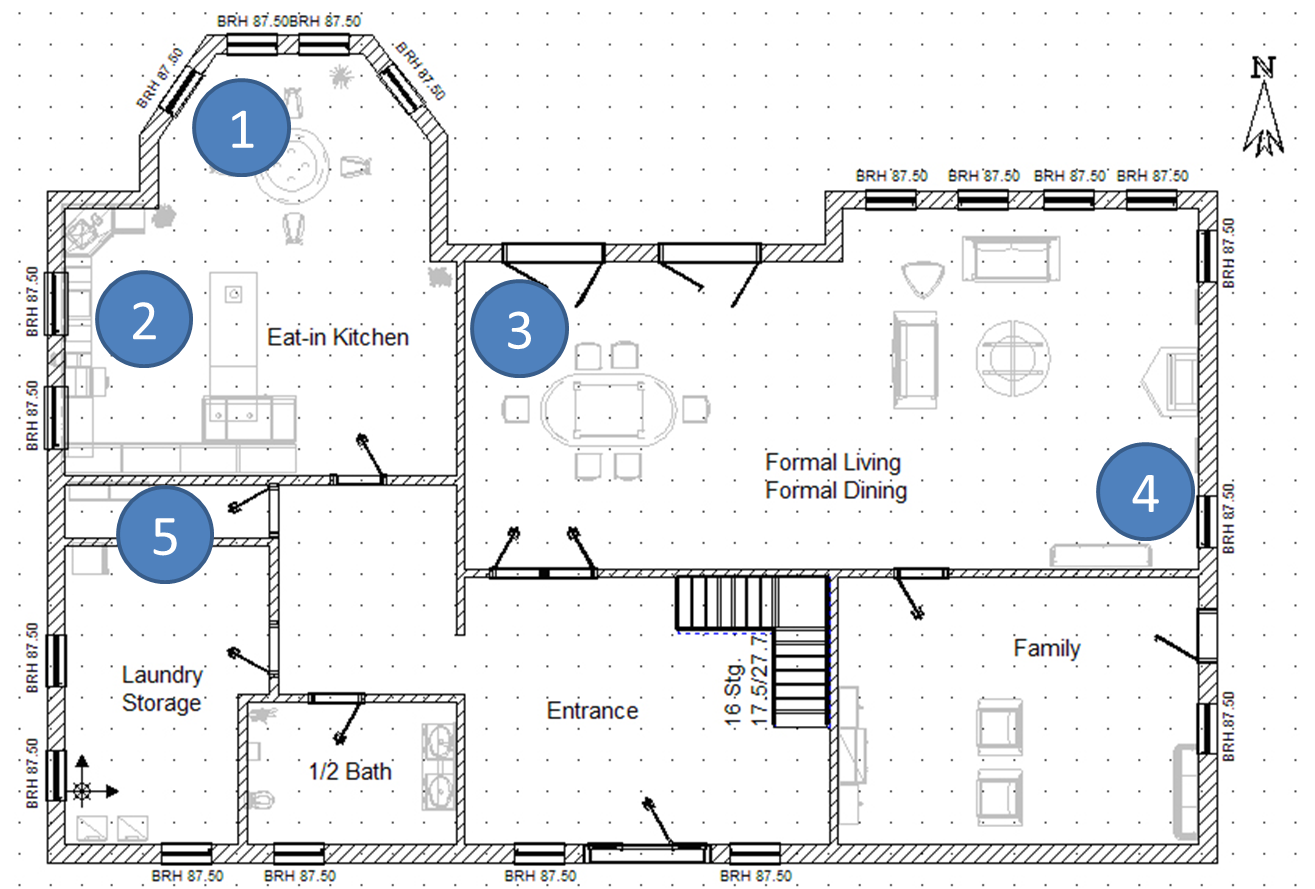
\includegraphics[scale=0.3]{house_floorplan.png}
%\caption{Example home floor plan showing five deployed temperature sensors} \label{house_floorplan}
%\label{fig:example_home_floorplan}
%\vspace{-0.1in}
%\end{figure}

\paragraph{Spatio-Temporal methods}
{\em Spatio-temporal methods} consider both the
temporal and spatial correlation; salient methods include
STI~\cite{Jian-Zhong:STI}, DESM~\cite{li2008data}, 
AKE~\cite{pan2010k}, and Imputation Method~\cite{Lim:robust}.
%These
%have the potential advantage of using both types of correlation in
%imputation, but can suffer from the spatial correlation issues
%discussed above.

The Spatial and Temporal Imputation (STI) algorithm is proposed in~\cite{li2008spatial}. 
For each missing record, STI first checks if some nodes are within the sensing neighborhood, and utilizes
the average of the neighbors to impute the missing value. If no sensors are within the neighborhood, the last seen value of the 
missing sensor is used for imputation. The method favors spatial information over temporal information.

%It has the advantage of simple and fast, but suffers when last seen value is far away from the current time stamp, or when most of the nodes in the sensing region has high missing rate.
%Furthermore, the usage of circular region is problematic as most of the landforms might not be uniformly distributed. Finally, determining the range of the radius is tricky, as a larger radius can cause noise while a smaller one cannot highlight the effectiveness of this model(i.e., the results will be similar to linear interpolation).
%The radius of the region is sometimes too large for sensors whose correlations with the target sensor are low in the sensing range.  
Another spatio-temporal algorithm is the Data Estimation using Statistical Model (DESM)~\cite{li2008data} method.  
In DESM, the prediction of a missing record is the linear combination of the previous reading of the sensor and the current reading of the neighboring sensor. The weight is given by Pearson correlation.

%Given two sensors data streams, $\{X_{i1},X_{i2},\dots,X_{im}\}$ and \\ $\{X_{j3},X_{j2},\dots,X_{jm}\}$, and assuming
%the value of $X_{i(m+1)}$ is missing,
%the prediction on sensor $i$ by its nearest sensor $j$ is:
%\begin{center}
%$\hat{X}_{i(m+1)} = (1-\alpha)X_{im} + (\alpha)\hat{z}$
%\end{center}
%where $\alpha$ is the Pearson correlation coefficient between the sensor $i$ and $j$, and $\hat{z}$ is the estimation of sensor $i$ 
%based on the observation from sensor $j$---it measures the influence of the data sensed by node $i$ on the data of 
%the nearest node $j$:
%\begin{center}
%$\hat{z} = X_{im}(1+\frac{X_{j(m+1)}-X_{j(m)}}{X_{j(m)}})$
%\end{center}
%The above equation assumes that the sensor $X_i$ and $X_j$ have the similar data fluctuation trend. 
%$\alpha$ is expected to have more impact on the prediction if $X_i$ is more correlated with $X_j$. 
%\begin{equation}
%\label{z-hat}
%\end{equation}
%In DESM, because $\alpha$ is usually high around the target sensor. Therefore, the temporal feature multiplied by $1-\alpha$ holds a very small portion of contribution to the prediction process. It often contradicts the nature that the temporal correlation itself is usually higher than any spatial correlation with other sensors. The performance may becomes bad if the nearest sensor is not the most correlated one, i.e., blocked by a wall.
% \subsubsection{Applying K-nearest neighbour Estimation}

K-nearest neighbors algorithm (KNN) is an intuitive yet effective spatial-correlation-based imputation method. 
It directly uses the weighted average of the neighbor signals to impute the missing data, and has been adopted to successfully 
estimate the missing values of DNA micro-arrays~\cite{Troyanskaya:DNAKNN}.  
%While in WSNs, the sensor data of different nodes is more likely to have some functional relations other than just using sensor values.
Pan~\cite{pan2010k} proposes the Applying K-nearest neighbor Estimation (AKE) algorithm to exploit the spatial correlation in the 
missing sensory data problem. 
AKE adopts a linear regression model to describe the spatial correlation of nodes $i$ and $j$,
%\begin{center}
$y_{it} = \alpha + \beta\cdot y_{jt} + \mu_{jt} $,
%\end{center}
where $y_{it}$ is the observation of sensor $i$ at time $t$, $y_{jt}$ is the data of sensor $j$ at the same time, 
and $\mu_{jt}$ is the random error at time t.   
When the data of sensor $i$ at time $t$ is missing, the estimated value of sensor $i$ by sensor $j$ at the same time is:
%\begin{center}
$\hat{y}_{it}^{(j)} =\hat{\alpha} +\hat{\beta}\cdot y_{jt}$
%\label{ake_j}
%\end{center}
The $\hat{\alpha}$ and $\hat{\beta}$ are the estimated values of $\alpha$ and $\beta$, based on the sample data according to the least squares principle.
%They claim that using a linear combination of the estimation from neighbour sensors can lower the random error caused by only using a single sensor. 
Therefore, given the $m$ nearest neighbor sensors who have values at time $t$[$y_{1t}, y_{2t},\dots, y_{mt}$], the missing value is predicted by :   
% \begin{center}
$ \hat{y}_{it} =\sum_{j=1}^m w_j \cdot \hat{y}_{it}^{(j)}$
 %\label{ake_impute}
% \end{center}
% First they build a matrix 
%\[ \left( \begin{array}{cccc}
%
%\end{array}
%\right)
%\]
where $w_j$ is the weight of sensor $j$ used to predict sensor $i$, and is larger for more highly correlated pairs.
%They adopt the r-square statistics to rank their correlations. The value of $w_j$ is the weighted average of the corresponding 
%r-square values for the $m$ sensors. 

The above models suffer from an issue as they make some unverified assumptions about the data. For example, some models consider temporal correlation as more important than spatial correlation,
%such that the reading of nearby sensors are used only when nearby time steps are missing (or vice versa),
while some assume that sensors of the same distance should have a similar correlation regardless of their 
orientation or other factors.  Such assumptions might or might not hold for various types of data, while imposing them a priori
to the model build might lead to inconsistent results.  The models we propose, however, try to rely less on such a priori 
knowledge, and learn the latent correlation directly from the data.  
%The Imputation Method (ImM)~\cite{Lim:robust}, tries to learn
%the appropriate weighting of temporal and spatial features by considering two temporal predictors, the last-seen predictor
%and an autocorrelation-based temporal linear predictor, and one spatial linear predictor.

\paragraph{Singular Value Decomposition (SVD)-based Methods}
Among the spatio-temporal methods, some are Singular Value Decomposition (SVD)-based methods which are conceptually closer to our
solution. 
SVD-based methods have a significant limitation as they can only be applied to a complete matrix.
Therefore, one needs to somehow first fill in the missing values before conducting such decomposition.
The initial assignment of those missing values, unfortunately, can significantly affect the performance~\cite{koren2009matrix}.
Furthermore, SVD is computationally expensive in general.
In contrast, our approach relies on the factorization process on an incomplete matrix.

%SVD is widely used as a dimension reduction technique.
%It decomposes a fully observed matrix~$\mathbf{R}$ into one diagonal matrix~$\mathbf{D}$ and two unitary matrices~$\mathbf{U}$ and~$\mathbf{V}$ such that
%$\mathbf{R} = \mathbf{U}\mathbf{D}\mathbf{V}^T.$
%The largest $K$ singular values and vectors, $\mathbf{U}_K \mathbf{D}_K \mathbf{V}_K^T$, form the best $K$-rank approximation of $\mathbf{R}$ under the Frobenius Norm.

A salient example of SVD-based approaches for imputation is the Empirical Orthogonal Functions
(EOF) model, which has been applied to oceanographic applications to
solve the problem of missing or unreliable satellite
data~\cite{beckers2003eof}.  EOF first fills in the missing values
(e.g., using all zeros or the mean values) and then performs SVD 
to decompose the matrix. The first $K$ spatial-EOF (i.e., the top-$K$
singular values in SVD) is used to reconstruct the matrix and update the estimation of missing values, 
where $K$ is determined through cross validation over the data.

%In the field of Collaborative Filtering, researchers have already pointed out
%several drawbacks in the SVD-based methods. % when applying to impute missing data. 
%First, given large data, it
%is computational demanding as we need to do the decomposition
%in every iteration. Second, it requires to fill in all missing values
%before the decomposition can be performed, and imperfect initial
%imputation can significantly hurt the final imputation results, in
%particular when the missing data rate is
%high~\cite{koren2009matrix}.

%Hybrid methods of temporal and spatial approaches are less common in the literature.
%For example, the average of the temporal approach of linear interpolation and the spatial approach of multivariate regression has been reported[8].
%Strictly speaking, this approach can be thought of as an ensemble approach between the two methods rather than a fully-integrated approach which considers both temporal and spatial aspects of WSN data.

%\subsection{Research Gap Identification (why are current approaches inadequate?)}
%Accurate imputation of missing sensor network observations is crucial to allow for effective subsequent analysis.
%While there are many existing algorithms which estimate missing data (as documented in the following Related Works section), few of these take advantage of the time and space dependencies inherent in the WSN datasets during the data imputation process.
%As a result, the accuracy of such approaches is limited.

%\subsection{Method Overview \redtext{(what is our approach to bridge the research gap?)}}

\subsection{Our Approach: Collaborative Filtering}

In this paper, we employ a novel {\em Collaborative Filtering} (CF) approach
to sensor data imputation inspired by the field of Recommendation
Systems.  In typical CF approaches, the elements of interest are users
and items (e.g., products), and the values are user ratings of those
items (as in the left-hand side of
Figure~\ref{recommend_imputation}).  Typically, most of the ratings
are missing, and the goal is to predict (impute) the missing ratings
in order to ``recommend'' items to users.  By viewing sensors as
items, users as time steps, and readings as ratings (as illustrated in
Figure~\ref{recommend_imputation}), we can apply CF
techniques to perform sensor data imputation. (Alternatively, sensors
can be viewed as users and items as time steps---the mapping is
irrelevant to the CF formulation.)  In particular, we focus on the
widely successful {\em Matrix Factorization} (MF) technique for CF.

\begin{figure}[H]
\centering
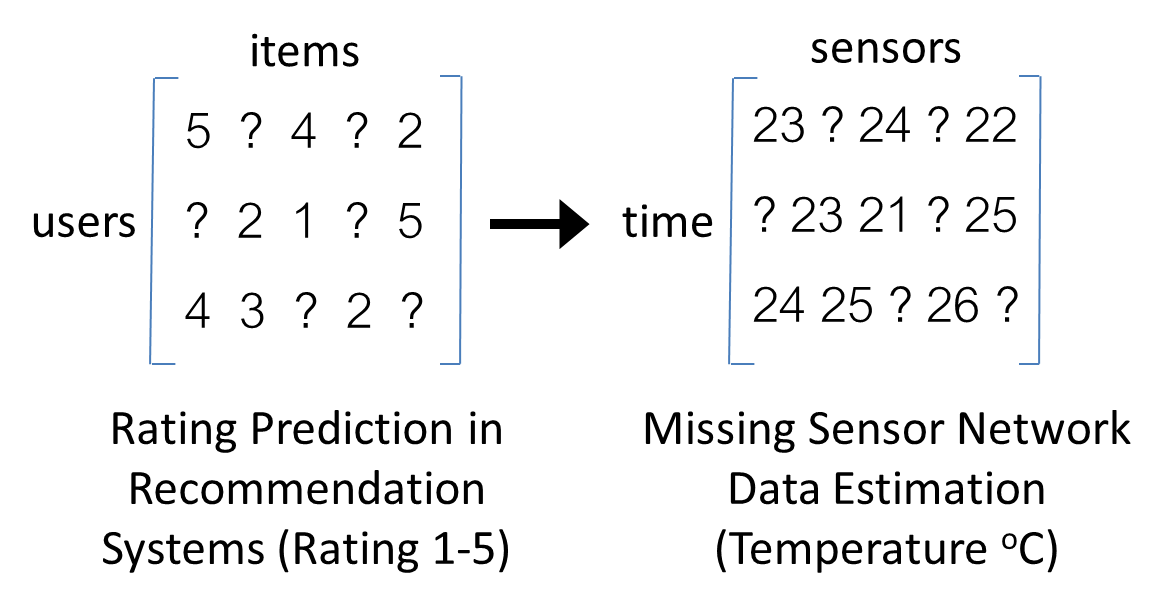
\includegraphics[scale=0.35]{recommend_imputation_timerow.png}
\caption{Bridge from Recommendation Systems to Sensor Data Imputation} 
\label{recommend_imputation}
\vspace{-0.1in}
\end{figure}

Sensor readings differ from user ratings, however, in that the former
exhibit high correlation in both time and space (subject to the above
caveats on space).  To incorporate this property, we first modify MF
to model temporal correlations and learn latent relationships among
sensors.  Specifically, we add temporal-proximity terms to
MF---we call this {\em Temporally-Regularized MF} (TR-MF). 
Similarly, we can also add spatial-proximity terms---we 
call this {\em Spatially-Temporally-Regularized} MF (STR-MF).

Second, we consider sensor networks with multiple sensor types at each node.
We are readily able to exploit such heterogeneous sensor information in our
solution, in contrast to most prior imputation methods that use more ad hoc means.
%Our method incorporates these heterogeneous sensor
%signals (for example, estimating the temperature at a given sensor
%node utilizing the humidity and temperature trends from other
%sensors in the network) to provide more accurate imputation than 
%prior approaches.
We present two techniques for extending 
TR-MF to account for possible correlations among sensor types: {\em Multivariate TR-MF} and 
{\em Temporally-Regularized Tensor Factorization} (TR-TF).

We evaluate our approaches using two environmental sensor network
datasets, one indoor and one outdoor.
%Both datasets record temperature, humidity, and light within its deployed
%environment.  Each dataset has a roughly 50\% initial missing rate (strengthening
%the claim that missing data in WSNs is a common issue), to which we
%additionally cover known observations to use for validation and
%testing purposes.
We study two patterns for missing data: (i) covering
{\em random} readings (modeling intermittent reading failures) and (ii)
covering {\em consecutive} readings for some sensor nodes
(modeling long temporal gaps such as with failed sensors).

Our study shows that TR-MF provides significantly higher estimation accuracy than 
both (i) state-of-the-art recommendation models and (ii) state-of-the-art sensor data imputation approaches 
such as AKE (which is the most accurate prior spatio-temporal method).
Furthermore, our study shows that STR-MF, which adds spatial coordinate information into TR-MF, 
is useful {\em only} in the ``consecutive'' pattern---perhaps surprisingly,
STR-MF is significantly {\em less} accurate than TR-MF in the ``random'' pattern.  This is because TR-MF
effectively leverages the latent relationships among sensors, including any spatial correlations, while avoiding the
pitfalls of spatial-proximity biases.

For the heterogeneous setting, our study shows that both
Multivariate TR-MF and TR-TF can significantly improve the accuracy over TR-MF,
and each has its strengths, depending on the observed variance in the
readings.  Finally, we consider a popular data analysis task---building regression-based prediction models---and show that,
compared to prior approaches for imputation, using TR-MF leads to a much higher quality prediction model.

These results validate our novel approach of equating sensor imputation with recommendation systems.  
%CF approaches such as Matrix Factorization and Tensor Factorization are adept at handling scenarios 
%with large numbers of missing values.
Correlations are captured by grouping correlated sensor nodes and correlated time
steps---unlike prior sensor data imputation approaches, our CF
approaches use this {\em latent} information to impute values, and optimize the evaluation metrics directly. 
Moreover, our CF approaches are global, taking into account all
collected observations, and not overly tied to spatial-proximity
correlations.  
%For example, they can capture the correlations between
%distant sensors $3$ \& $4$ in Figure~\ref{house_floorplan}, while
%grouping sensors $1$, $2$ \& $5$ only if the observed readings warrant
%it.  The CF framework also provides a unified approach to incorporate
%any number of additional sensor types for an even more accurate imputation.

%The reason we believe our method outperforms the results of other methods are as follows.
%\begin{itemize}
%\item A CF approach utilizes {\em latent} information between sensors, e.g., inter-sensor correlation
%\item utilizing heterogeneous sensor information (e.g., utilizing humidity information when estimating temperature) provides additional features which enables a more refined estimation model
%\item we provide an efficient optimization method to learn the inherent model parameters effectively
%\item our method provides a global solution, where all sensor observations available in the dataset can potentially aid in the estimation of a given missing observation
%\end{itemize}

% Given these experimental conditions, we show that our temporal and spatial-oriented collaborative filtering approach to data imputation for WSNs performs more accurately than existing methods such as linear regression and hybrid-kNN.
% In Matrix Factorization, we impose the temporal regularization and Temporal-Regularied MF show the best performance compared to all competitor algorithmss.
% On top of that, we add in spatial regularization and multivariate learning, and we discuss under which circumstance these two are applicable and how they can even improve our models.
% We propose the Tensor Factorization model for missing data recovery. The TF model use additional dimension to capture the correlations of features such as temporal, spatial or heterogeneous signal correlations. The conventional Tensor decomposition technology can only apply on dense tensor. The study of Tensor Factorization model in Collaborative Filtering for recommendation recently, but not practical in sensor network. We  have adapted the TF model for missing value estimation. 

\subsection{Contributions}

In summary, the main contributions of this paper are:
\begin{itemize}
\item We propose viewing sensor data imputation as a recommendation systems problem, and apply state-of-the-art collaborative filtering methods of recommendation systems (namely, matrix and tensor factorization) to the sensor network domain.
\item We augment collaborative filtering with temporal regularization and multi-sensor signals, and provide efficient optimization methods to learn the inherent model parameters effectively.
\item We present an empirical study on two sensor datasets, considering two
missing data patterns corresponding to intermittent readings and failed
sensors. The results show that our proposed approaches provide
significantly higher estimation accuracy than state-of-the-art prior
approaches, and moreover, such accuracy improvements can result in the
generation of higher-quality prediction models.
\end{itemize}

% which finds that our method works well without the incorporation spatial information and that our approach can facilitate the generation of better prediction models

%\subsection{Paper Organization}

%\noindent{\bf Roadmap.}
%%The remainder of our paper is organized as follows.  
%Related work is reviewed in Section~\ref{sec:rw}.  In Sections~\ref{sec:mf} and~\ref{sec:tf} 
%we describe our factorization and multivariate factorization
%approaches to sensor data imputation, respectively. Section \ref{sec:exp} presents our experimental study. 
%Sections \ref{sec:disc} and \ref{sec:conc} provide discussions of our findings and conclusions.
